\documentclass{article}

% --- packages ---

\usepackage[utf8]{inputenc}
\usepackage[english, ngerman]{babel}
\usepackage{amsmath}
\usepackage{booktabs}
\usepackage{amsthm}
\usepackage{mathdots}
\usepackage[linesnumbered,ruled,noline]{algorithm2e}
\usepackage{tikz, pgfplots}
\usepackage{amssymb}
\usepackage{graphicx}
%\usepackage{subcaption}
\usepackage{multirow}
\usepackage{pgf}
\usepackage{caption}
\usepackage{listings, lstautogobble}
\usepackage{delarray}
\usepackage{bigints}
\usepackage{float}
\usepackage{layouts}
\usepackage{subfigure}
\usepackage{url}
\usepackage{fancyhdr}
\usepackage{MnSymbol}
\usepackage{wasysym}
\usepackage[a]{esvect} %für bessere Vektorpfeile
\usepackage{setspace}
\usepackage{geometry}
\usepackage{hyperref}
\usepackage{array}
\usepackage{acronym}
\usepackage{ifsym}
\usepackage[sorting=nty]{biblatex}
\usepackage[nottoc,numbib]{tocbibind}

% --- Input macros von Ide ---

%\input{macros}

% --- Seitenränder / Einrücktiefe ---

\geometry{left=2.5cm, right=2.5cm, top=2cm, bottom=2cm}
\parindent0cm

% --- new commands ---

\newcommand{\RM}[1]{\MakeUppercase{\romannumeral #1{}}} %für römische Zahlen #1{}}} %für römische Zahlen
\newcommand{\xvec}{\underline{x}}
\newcommand{\bvec}{\underline{b}}
\newcommand{\uvec}{\underline{u}}
\newcommand{\vvec}{\underline{v}}
\newcommand{\wvec}{\underline{w}}
\newcommand{\pvec}{\underline{p}}
\newcommand{\zvec}{\underline{z}}
\newcommand{\xstern}{\underline{x}^*}
\newcommand{\Rmn}{\mathbb{R}^{m \times n}}
\newcommand{\Elasticsearch}{\textit{Elasticsearch}\;}
\newcommand{\Rnn}{\mathbb{R}^{n \times n}}
\newcommand{\rang}{\text{rang}}
\def\code#1{\texttt{#1}}
\newcommand{\dom}{\textrm{dom}}
\newcommand{\lojoin}{{\tiny \textifsym{d|><|}}}
\newcommand{\rojoin}{{\tiny \textifsym{|><|d}}}
\newcommand{\fojoin}{{\tiny \textifsym{d|><|d}}}
\newcommand{\m}{\cdot} %Malzeichen einfacher
\newcommand{\entspricht}{$\mathop{\hat{=}}$} %Entspricht-Zeichen
\renewcommand{\labelnamepunct}{\addcolon\space}

% -- Definitionen für Theoremumgebungen ---

\newtheoremstyle{newline}% name
{}% Space above
{\baselineskip}% Space below
{\normalfont}% Body font
{}% Indent amount
{\bfseries}% Theorem head font
{:}% Punctuation after theorem head
{\newline}% Space after theorem head
{\thmname{#1}\thmnumber{ #2}\thmnote{ (#3)}}% Theorem head spec (can be left empty, meaning ‘normal’ )

\theoremstyle{newline}
\newtheorem{definition}{Definition}[section]
\newtheorem{satz}[definition]{Satz}
\newtheorem{bemerkung}[definition]{Bemerkung}
\newtheorem{folgerung}[definition]{Folgerung}

\renewenvironment{proof}[1][\proofname:]{%
\minisec{#1}
\pushQED{\qed}%
\itshape
}{%
\popQED
\par
\medskip
}

% --- listing_settings ---
\lstset{
	language=Python,
	frame=single, % Rahmen um den Code
	numbers=left, % Zeilennummern auf der linken Seite
	numberstyle=\small, % Stil der Zeilennummern
	xleftmargin=2em, % Abstand zum linken Rand
	keywordstyle=\color{blue}, % Kewyord Style
	tabsize=4,
	breaklines=true,
}

% --- options for algorithm
\SetKwComment{Comment}{/* }{ */}


% --- Define colors ---

\definecolor{red}{rgb}{0.6,0,0} % for strings
\definecolor{blue}{rgb}{0,0,0.6}
\definecolor{green}{rgb}{0,0.8,0}
\definecolor{cyan}{rgb}{0.0,0.6,0.6}
\newcommand{\greencomment}[1]{\textcolor{green}{#1}}


\lstset{autogobble=true}

% --- Literaturverzeichnis ---
\bibliography{nserl.bib}


% --- Beginn des eigentlichen Dokuments ---


\begin{document}

% -- Layout Kopfzeile ---

\pagestyle{fancy}
\lhead{\small{\slshape}}
\chead{}	
\rhead{\mdseries \leftmark}


\begin{titlepage}

%\includegraphics[width=0.20\textwidth]{Bilder/fh_logo.png}\hfill\includegraphics[width=0.25\textwidth]{Bilder/diamant-software-logo-teams.png}

% --- include correct images here

\centering

{\bfseries HSBI Bielefeld \par}
\vspace{0.25cm}
{\bfseries University of Applied Sciences \par}
\vspace{0.25cm}
{\bfseries Fachbereich Ingenieurwissenschaften und Mathematik \par}
\vspace{0.25cm}
{\bfseries Studiengang Optimierung und Simulation \par}
\vspace{1.5cm}
{\huge\bfseries Lösen von nichtlinearen Gleichungssystemen mit einem Reinforcement-Learning-Agent \par}
\vspace{2.5cm}
{\Large\bfseries Bericht \par}
{\vspace{8.5cm}}

\flushleft
\begin{tabular}{ll}
	Vorgelegt von: & Nicolas Schneider \vspace{0.25cm}\\
	Matrikelnummer: & 1208960 \vspace{0.25cm} \\
	Studiengang: & Optimierung und Simulation \vspace{0.5cm} \\
	Abgabedatum: & 07.04.2024 \vspace{0.5cm} \\
	Betreuer: & Prof. Dr. rer. nat. Bernhard Bachmann
\end{tabular}
\vfill
\end{titlepage}


\thispagestyle{empty}
\newpage



\begin{onehalfspace}

\thispagestyle{empty}
\selectlanguage{english}
\begin{abstract}
	Nichtlineare Gleichungssysteme (NGS) spielen eine zentrale Rolle in vielen Bereichen der Wissenschaft und Technik, da sie zur Modellierung und Lösung komplexer Probleme in Physik, Chemie, Ingenieurwesen und anderen Disziplinen eingesetzt werden. Trotz ihrer Bedeutung stellt die Lösung von NGS aufgrund ihrer inhärenten Nichtlinearität und des Fehlens geschlossener analytischer Lösungen eine große Herausforderung dar. Traditionelle numerische Verfahren wie das Newton-Raphson-Verfahren oder Optimierungsansätze stoßen oft an ihre Grenzen, insbesondere bei hochdimensionalen Problemen, chaotischem Verhalten oder starker Abhängigkeit von Anfangsbedingungen.
	
	In jüngster Zeit hat der Bereich des Reinforcement Learnings (RL) zunehmend an Bedeutung gewonnen und vielversprechende Ergebnisse bei der Lösung komplexer Probleme geliefert. RL-Agenten lernen durch Interaktion mit einer Umgebung und Belohnungssignale, optimale Strategien zu entwickeln, ohne explizite Programmierung. Dieser Ansatz hat sich in verschiedenen Anwendungsfeldern wie Robotik, Spielen und Optimierungsproblemen als erfolgreich erwiesen.
	\\
	
	In dieser Arbeit wird der Ansatz des RL verwendet, um Lösungen für nichtlineare Gleichungssysteme zu finden. Ein RL-Agent wird in einer maßgeschneiderten Umgebung trainiert, die die Struktur des gegebenen nichtlinearen Gleichungssystems widerspiegelt. Durch die Formulierung von Belohnungen für Aktionen, die den Agenten näher an eine Lösung führen, wird dieser befähigt, iterative Strategien zur effizienten Lösungsfindung zu erlernen.
	
	Die vorliegende Arbeit präsentiert einen initiierenden Ansatz und analysiert seine Leistung hinsichtlich Schnelligkeit und Genauigkeit bei der Lösungsfindung von nichtlinearen Gleichungssystemen. Dabei wird eine erste Untersuchung durchgeführt, um die Effektivität dieses Ansatzes im Vergleich zu etablierten Methoden wie dem Newton-Raphson-Verfahren zu bewerten. Besonderes Augenmerk wird auf die Identifizierung und Analyse der limitierenden Faktoren dieses Ansatzes gelegt, um potenzielle Schwächen aufzudecken und zu verstehen, inwiefern dieser Ansatz für praktische Anwendungen geeignet ist.
	
	% Hier noch Ergebnisse kurz darstellen?
	
\end{abstract}
\selectlanguage{ngerman}
\newpage


\tableofcontents	% Inhaltsverzeichnis		
\thispagestyle{empty}

\newpage		

\section{Grundlagen nichtlinearer Gleichungssysteme}

Ein nichtlineares Gleichungssystem kann als Nullstellenproblem wie folgt formuliert werden:

\begin{definition}[Nichtlineares Gleichungssystem]
	Es sei $B \subset \mathbb{R}^n$ und $\mathbf{g}: B \rightarrow \mathbb{R}^n$. Gesucht sind Lösungen von
	
	\begin{center}
		$\mathbf{f}(\mathbf{x}) = \mathbf{0}.$
	\end{center}
	
	$\mathbf{f}(\mathbf{x}) = \mathbf{0}$ ist ein System von $n$ nichtlinearen Gleichungen für $n$ Unbekannte $x_1, \dots, x_n$.
	\\
	
	\begin{center}
		\boxed{
			\begin{array}{ccc}
				f_1(x_1, \dots, x_n) & = &0\\
				f_2(x_1, \dots, x_n) & = & 0\\
				\vdots &&\\
				f_n(x_1, \dots, x_n) & = & 0
			\end{array}
		}
	\end{center}
	\cite{Merzigera}
\end{definition}
\bigskip

Nichtlineare Gleichungssysteme treten in vielen Bereichen der Wissenschaft und Technik auf, wie beispielsweise in der Physik, Chemie, Biologie, Wirtschaftswissenschaften und Ingenieurwissenschaften. Sie dienen zur Modellierung und Analyse komplexer Systeme, deren Verhalten durch nichtlineare Beziehungen zwischen den Variablen beschrieben wird.

Die Lösung solcher Systeme ist jedoch oft eine große Herausforderung, da nichtlineare Gleichungen im Allgemeinen keine geschlossenen analytischen Lösungen besitzen und zu den $NP$-schweren Probleme zählen. Stattdessen müssen numerische Verfahren eingesetzt werden, um approximative Lösungen zu finden. Einige gängige Methoden zur Lösung nichtlinearer Gleichungssysteme sind:

\begin{enumerate}
	\item \textbf{Iterative Verfahren}: Hierzu zählen Methoden wie das Newton-Raphson-Verfahren, das Quasi-Newton-Verfahren und das Broyden-Verfahren. Diese Verfahren starten mit einer Anfangsschätzung und verbessern diese iterativ, bis eine ausreichend genaue Lösung gefunden ist.
	
	\item \textbf{Globale Optimierungsverfahren}: Wenn das Gleichungssystem als Optimierungsproblem formuliert werden kann, können globale Optimierungsverfahren wie die Branch-and-Bound-Methode oder evolutionäre Algorithmen zur Lösung eingesetzt werden.
\end{enumerate}

Die Schwierigkeit, nichtlineare Gleichungssysteme zu lösen, besteht oft darin, geeignete Anfangsschätzungen für die Iterationsverfahren zu finden und die Konvergenz der Verfahren sicherzustellen. Viele Systeme weisen mehrere Lösungen auf, von denen einige instabil oder nicht physikalisch sinnvoll sein können. Darüber hinaus können nichtlineare Systeme eine komplexe Struktur mit mehreren lokalen Extrema aufweisen, was die globale Konvergenz erschwert. 


\section{Grundlagen Reinforcement Learning}

Reinforcement Learning (RL) ist ein Teilgebiet des Maschinellen Lernens, bei dem ein Agent lernt, durch Interaktion mit einer Umgebung eine bestimmte Aufgabe oder ein Ziel zu erreichen. Im Gegensatz zu überwachtem Lernen, bei dem ein Modell anhand von Trainingsbeispielen mit bekannten Eingabe-Ausgabe-Paaren gelernt wird, erhält der Agent beim Reinforcement Learning nur eine skalare Bewertung (Reward) für seine Aktionen. Durch Ausprobieren und Lernen aus den erhaltenen Rewards versucht der Agent, eine Strategie (Policy) zu finden, die die kumulative Belohnung über die Zeit maximiert.
\\

\textbf{Markov-Entscheidungsprozess:}
\smallskip

Reinforcement Learning Probleme werden häufig als Markov-Entscheidungsprozesse (Markov Decision Processes, MDPs) formuliert. Ein MDP besteht aus:

\begin{itemize}
	\item Einem Zustandsraum $\mathcal{S}$, der alle möglichen Zustände der Umgebung enthält.
	\item Einem Aktionsraum $\mathcal{A}$, der alle möglichen Aktionen des Agenten definiert.
	\item Einer Übergangswahrscheinlichkeitsfunktion $\mathcal{P}(s, a, s')$, die die Wahrscheinlichkeit angibt, dass der Agent beim Ausführen der Aktion $a$ im Zustand $s$ in den Zustand $s'$ übergeht.
	\item Einer Belohnungsfunktion $\mathcal{R}(s, a, s')$, die die Belohnung definiert, die der Agent erhält, wenn er aus dem Zustand $s$ durch Ausführen der Aktion $a$ in den Zustand $s'$ übergeht.
\end{itemize}

Das Ziel des Agenten ist es, eine Policy $\pi: \mathcal{S} \rightarrow \mathcal{A}$ zu finden, die die erwartete kumulative Belohnung über die Zeit maximiert.

Abbildung \ref{fig:rl_grundlagen} stellt den Lernprozess eines Agenten in einer Umgebung vereinfacht dar.

\begin{figure}[h]
	\centering
	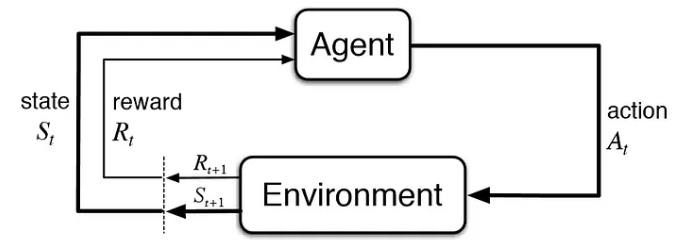
\includegraphics[width=0.5\textwidth]{Bilder/rl_grundlagen.png}
	\caption{Vereinfachter Lernprozess eines Agenten in einer Umgebung\protect\footnotemark}
	\label{fig:rl_grundlagen}
\end{figure}
\footnotetext{\url{https://towardsdatascience.com/reinforcement-learning-101-e24b50e1d292}}


\textbf{Value Functions und Bellman-Gleichungen:}
\smallskip

Eine zentrale Rolle beim Reinforcement Learning spielen die Value Functions, die den erwarteten kumulativen Reward für einen gegebenen Zustand oder eine Zustand-Aktions-Paar angeben. Es gibt zwei wichtige Value Functions:

\begin{itemize}
	\item Die State-Value Function $V^\pi(s)$ gibt den erwarteten kumulativen Reward an, wenn der Agent im Zustand $s$ startet und der Policy $\pi$ folgt.
	\item Die Action-Value Function $Q^\pi(s, a)$ gibt den erwarteten kumulativen Reward an, wenn der Agent im Zustand $s$ startet, die Aktion $a$ ausführt und danach der Policy $\pi$ folgt.
\end{itemize}

Die Value Functions erfüllen die Bellman-Gleichungen, die eine rekursive Beziehung zwischen den Value Functions benachbarter Zustände herstellen. Für die State-Value Function lautet die Bellman-Gleichung:

\begin{equation}
	V^\pi(s) = \mathbb{E}_\pi \left[ R(s, a, s') + \gamma V^\pi(s') \right]
\end{equation}

Und für die Action-Value Function:

\begin{equation}
	Q^\pi(s, a) = \mathbb{E}_\pi \left[ R(s, a, s') + \gamma \sum_{s'} \mathcal{P}(s, a, s') V^\pi(s') \right]
\end{equation}

Hier ist $\gamma \in [0, 1]$ der Diskontierungsfaktor, der bestimmt, wie viel Gewicht zukünftigen Rewards beigemessen wird. Ein Wert von $\gamma$ nahe 0 bedeutet, dass der Agent nur die unmittelbaren Rewards optimiert, während ein Wert nahe 1 längerfristige Belohnungen stärker gewichtet. (vgl. \cite{Lia2022})
\\

Dieses Kapitel bietet eine grundlegende Einführung in das Reinforcement Learning (RL), einem Teilgebiet des Maschinellen Lernens. RL ermöglicht es einem Agenten, durch Interaktion mit seiner Umgebung eine bestimmte Aufgabe zu erlernen, indem er Belohnungen für seine Aktionen maximiert, ohne explizite Trainingsdaten zu erhalten.

Der Markov-Entscheidungsprozess (MDP) bildet den Kern eines RL-Problems, definiert durch einen Zustandsraum, einen Aktionsraum, eine Übergangsfunktion und eine Belohnungsfunktion. Dabei spielen Value Functions und Bellman-Gleichungen eine entscheidende Rolle, um den erwarteten kumulativen Reward zu bewerten.

Es ist wichtig zu betonen, dass die Umsetzung eines RL-Agenten stark vom Anwendungsfall und den verfügbaren Daten abhängt, was zu einer großen Variabilität in der Implementierung führt. Dieses grundlegende Verständnis dient als Ausgangspunkt für die weiterführende Diskussion darüber, wie RL bei der Lösung nichtlinearer Gleichungssysteme eingesetzt werden kann. 

\section{Reinforcement Learning für die Lösung nichtlinearer Gleichungssysteme}

Bevor ein RL-Agent nichtlineare Gleichungssysteme lösen kann, sollten zunächst einige wichtige Fragen beantwortet werden, die für die Qualität der Lösung und die Lösungsfindung von Relevanz sind:

\begin{enumerate}
	\item \textbf{Umgebung:} Was ist die Umgebung, in dem der Agent agiert?
	\item \textbf{Zustand:} Was sind zulässige und sinnvolle Zustände?
	\item \textbf{Aktionen:} Was sind zulässige und sinnvolle Aktionen, die der Agent wählen kann?
	\item \textbf{Belohnung:} Wie sieht eine zielführende Belohnungsfunktion aus?
\end{enumerate}

Diese Projektarbeit fokussiert sich auf einen ersten Ansatz, der hinsichtlich seiner Effektivität untersucht wird.

Für die oben genannten Fragen wurden folgende erste Lösungsansätze entwickelt:
\\

\underline{Umgebung:}
\smallskip

Im Kontext dieses Projekts wird die Umgebung als der Raum betrachtet, in dem sich die Gleichungen befinden. Ein besonderes Merkmal dabei ist, dass die Umgebung als statisch betrachtet werden kann, sofern sich die Gleichungen und damit einhergehend auch die Lösungen während des Lösungsprozesses nicht ändern.
\\

\underline{Zustand:}
\smallskip

Der Zustand wird aufgefasst, als die gewählte Aktion.
\\

\underline{Aktion:}
\smallskip

Abhängig von der Dimensionalität des Problems kann der Agent aus einem kontinuierlichen Raum von Punkten wählen. Der Agent wählt eine Aktion $a \in \mathcal{A}$, wobei $\mathcal{A} \subseteq \mathbb{R}^{n-1}$ und $n$ die Dimensionalität des Problems widerspiegelt.
\\
 
\underline{Belohnungsfunktion:}
\smallskip

Die Formulierung der Belohnungsfunktion konzentriert sich darauf, die Lösung(en) des Gleichungssystems zu finden, sofern sie denn existieren. In dieser Arbeit wird das Residuum verwendet, welches den Fehler zur eigentlichen Lösung darstellt. Das Residuum $R$ an der Optimallösung $x^{\ast}$ ist $0$, sodass das Ziel dabei ist diesen Fehler zu minimieren. 

\begin{definition}[Residuum]
	Gegeben seien $n$ nichtlineare Gleichungen mit $\mathbb{R}^n \rightarrow \mathbb{R}^n$. Es sei vorausgesetzt, dass mindestens eine Lösung $\mathbf{x}^{\ast}$ existiert, die das Gleichungssystem löst. Dann ist das Residuum an der Stelle $\mathbf{x}$ mit $\mathbf{x} \in \mathbb{R}^n$ definiert als
	
	\begin{equation}
		R(\mathbf{x}) = \sum\limits (f_i(\mathbf{x}) - f_j(\mathbf{x}))^2 \quad \forall 1 \leq i < j \leq n.
	\end{equation}
\end{definition}

Da der Agent das Ziel verfolgt die Belohnung über die Zeit zu maximieren, kann das negative Residuum als Belohnung interpretiert werden. Es gilt also: $Reward = -R(\mathbf{x})$.
\\

Dieses Kapitel soll die grundsätzlichen Fragen beantworten, die bei der Kombination von RL und nichtlinearen Gleichungssystemen auftreten können. Diese müssen vor der tatsächlichen Umsetzung unbedingt und mit Sorgfalt beantwortet werden, sodass eine zielführende Lösungsfindung garantiert ist.

Besonderes Augenmerk gilt dabei der Umgebung, dem Zustands- sowie Aktionsraum und der Belohnungsfunktion des Agenten.

Da die Grundlagen für nichtlineare Gleichungssysteme, sowie für RL gelegt worden sind, wird im nachfolgenden Kapitel der Frage nachgegangen, wie diese Problemstellung genau umgesetzt werden kann.

\section{Umsetzung}

Bevor mit der Implementierung der Problemstellung, der Umgebung und des Agents begonnen wird, ist es von entscheidender Bedeutung, die Auswahl der richtigen Programmiersprache und Bibliothek sorgfältig zu prüfen. Diese Entscheidung bildet das Fundament für das gesamte Projekt und kann einen erheblichen Einfluss auf die Effizienz, Skalierbarkeit und den Erfolg der Umsetzung haben.
\medskip

Für dieses Projekt wurde die Programmiersprache \textit{Python} als Programmiersprache gewählt, zusammen mit der Reinforcement-Learning-Bibliothek \textit{stable-baselines3}. Diese Entscheidung basiert darauf, dass \textit{stable-baselines3} eine breite Palette von wichtigen RL-Algorithmen implementiert und gleichzeitig eine benutzerfreundliche Integration mit \textit{Python} bietet. Außerdem bietet diese Bibliothek eine ausgezeichnete Kompatibilität mit der Programm-Bibliothek \textit{gymnasium} von OpenAI, die essensziell für Erstellung von RL-Umgebungen ist. Die Kombination aus \textit{Python}, \textit{stable-baselines3} und \textit{gymnasium} ermöglicht eine effiziente Entwicklung und Umsetzung von Reinforcement-Learning-Algorithmen für die gegebenen Anforderungen des Projekts (vgl. \cite{Raffin2021}, vgl. \cite{Towers2023}). Der Programm-Code kann im folgenden Repository eingesehen werden: \url{https://github.com/Nicolas2912/OuS_Projekt}.
\\

Für die Umsetzung des Agenten bzw. der Umgebung sind folgende Methoden für die Problemstellung relevant:

\begin{itemize}
	\item \textbf{\code{get\_distance(x)}}: Berechnet das Residuum für einen Vektor $\mathbf{x} \in \mathbb{R}^{n-1}$.
	\item \textbf{\code{reward(residuum, *args)}}: Berechnet den Reward basierend auf dem Residuum und weiteren zusätzlichen Parametern.
	\item \textbf{\code{step(action)}}: Führt einen Schritt während des Lernens in der Umgebung aus und aktualisiert dabei die Belohnung auf Grundlage verschiedener, vorher festgelegter Regeln.
	\item \textbf{\code{reset()}}: Setzt die Umgebung auf einen zufälligen Zustand zurück, sobald eine bestimmte Bedingung erfüllt ist.
\end{itemize}
\bigskip

Auch der RL-Algorithmus ist entscheidend für die Lösungsfindung, da er die Strategie bestimmt, nach der der Agent in der Umgebung handelt und lernt. Im Verlauf des Projekts wurden verschiedene Algorithmen aus der \textit{stable-baselines3}-Bibliothek getestet. Unter diesen hat sich der \textit{Proximal Policy Algorithmus} (PPO) als besonders geeignet für diese spezifische Problemstellung erwiesen.
\medskip

\underline{Umgebung:}
\smallskip

Neben vielen vorgegebenen Umgebungen, die in der Programm-Bibliothek \textit{gymnasium} implementiert sind wie z.B. \textit{Cart Pole}, \textit{Acrobot} oder \textit{Pendulum} ist es auch möglich eine eigene Umgebung für einen speziellen Anwendungsfall zu erstellen. Für die Problemstellung nichtlineare Gleichungssysteme mit einem RL-Agent zu lösen, wird eine eigene Umgebung erstellt. 

Nachfolgend ist eine verkürzte Initialisierung der Umgebung dargestellt.

\begin{lstlisting}[language=Python, caption={Initialisierung der Umgebung}, label={lst:python}]
	class CustomEnv(gym.Env):
		def __init__(self, dimension):
			super(CustomEnv, self).__init__()
			self.dimension = dimension
			self.low_bounds = -5.0 * np.ones(dimension)
			self.high_bounds = 5.0 * np.ones(dimension)
			self.action_space = gym.spaces.Box(low=self.low_bounds, high=self.high_bounds, dtype=np.float64)
			self.observation_space = gym.spaces.Box(low=-np.infty, high=np.infty, shape=(dimension,))
			self.state = np.array([random.uniform(self.x_min, self.x_max), random.uniform(self.y_min, self.y_max)] + [0.0] * dimension)	
\end{lstlisting}

Bei der Initialisierung der Umgebung muss der Bereich der möglichen Aktionen (\code{action\_space}) angegeben werden. Da mögliche Lösungen für ein nichtlineares Gleichungssystem sich im ganzen Raum $\mathbb{R}^n$ befinden können, bietet sich dieser auch für die möglichen Aktionen an. Jedoch ist es nicht möglich den ganzen Raum (von $-\infty$ bis $\infty$) anzugeben, sodass Grenzen gesetzt werden müssen. Diese sind im Code mit den Variablen \code{self.low\_bounds} und \code{self.high\_bounds} beschrieben. Hierbei zeichnet sich auch einer der Nachteile ab. Da bei den allermeisten nichtlinearen Gleichungssystemen von Beginn an nicht abzuschätzen ist, in welchem Teil des Lösungsraumes sich die Lösung(en) befindet/befinden, stellt die Wahl des Aktionsraumes auch eine Herausforderung dar. Ähnlich wie beim Newton-Raphson-Verfahren, bei dem ein initialer Startpunkt notwendig ist, der die Laufzeit des Verfahrens maßgeblich beeinflussen kann, so kann auch die Größe des Aktionsraumes die Laufzeit der Lösungsfindung maßgeblich beeinflussen.
\bigskip

\underline{Berechnung des Residuums (Distanz):}
\smallskip

Da die Qualität der aktuellen Lösung im Projektcode anhand des Residuums bestimmt wird, ist es wichtig, den Prozess der Residuum-Berechnung kurz darzustellen.
\medskip

Für manche Arten von Problemen hat es sich als vorteilhaft erwiesen, das Residuum auf eine festgelegte Skala zu skalieren (bspw. logarithmische Skalierung, Min-Max-Skalierung etc.). Im folgenden ist ein Ausschnitt aus der Methode zur Berechnung des Residuums zu sehen.

\begin{lstlisting}[language=Python, caption={Berechnung des Residuums}, label={lst:python}]
	def get_distance(point):
		scaling = "logarithmic"
		equations = self.nse()
		
		# Calculate the function values for all equations
		values = np.array([eq(point) for eq in equations])
		
		# calculate normal residuum
		normal_res = sum((values[i] - values[j]) ** 2 for i in range(len(values)) for j in range(i + 1, len(values)))
		self.all_residuals.append(normal_res)
		
		if scaling == "logarithmic":
			scaled_values = np.log1p(np.abs(values)) / np.log(10)
			res = sum((scaled_values[i] - scaled_values[j]) ** 2 for i in range(len(scaled_values)) for j in
			range(i + 1, len(scaled_values)))
			return res, normal_res		
\end{lstlisting}
\bigskip

\underline{Ausführung eines Lernschritts:}
\smallskip

Die Ausführung eines Lernschritts ist entscheidend für die Lösungsfindung und ist genauer in Algorithmus \ref{algo:step} beschrieben.

Zuerst seien die wichtigsten Variablen in Tabelle \ref{tab:Variablendefinition} definiert.

\begin{table}[htbp]
	\centering
	\caption{Variablendefinitionen}
	\label{tab:Variablendefinition}
	\begin{tabular}{>{\itshape}l p{0.6\linewidth}}
		\toprule
		\textnormal{Variable} & \textnormal{Beschreibung} \\
		\midrule
		\text{\code{distances}} & Eine Liste, die Entfernungen (Residuen) enthält. \\
		\text{\code{best\_actions}} & Eine Liste, die die besten Aktionen enthält. \\
		\text{\code{best\_distances}} & Eine Liste, die die besten erreichten Entfernungen enthält. \\
		\text{\code{improvement\_rate\_history}} & Eine Liste, die Verbesserungsraten enthält. \\
		\text{\code{good\_points\_threshold}} & Der Schwellenwert für einen \glqq guten Punkt\grqq{}. \\
		\text{\code{no\_improvement\_limit}} & Die Grenze für aufeinanderfolgende Iterationen ohne Verbesserung. \\
		\text{\code{dynamic\_reward}} & Die dynamisch akkumulierte Belohnung. \\
		\text{\code{dynamic\_penalty}} & Die dynamisch akkumulierte Strafe. \\
		\text{\code{total\_reward}} & Die insgesamt akkumulierte Belohnung. \\
		\text{\code{improvement\_rate}} & Die berechnete Verbesserungsrate. \\
		\text{\code{done}} & Ein boolescher Wert, der den Abschluss anzeigt. \\
		\text{\code{consecutive\_no\_improvement}} & Die Anzahl aufeinanderfolgender Iterationen ohne Verbesserung.\\
		\bottomrule
	\end{tabular}
\end{table}
\newpage

\begin{algorithm}
	\caption{Ausschnitt zur Ausführung eines Schrittes}
	\label{algo:step}
	\KwIn{action}
	\small
	\KwOut{reward, done}
	\SetKwData{residuum}{residuum}
	\SetKwData{threshold}{threshold}
	\SetKwData{distancesarray}{distances\_array}
	\SetKwData{improvementrate}{improvement\_rate}
	\SetKwData{return}{return}
	
	\SetAlgoSkip{2em} % Erhöht den vertikalen Abstand zwischen den Zeilen
	
	% Initialization
	\textbf{Initialization:}
	
	\text{\code{residuum}} = \code{get\_distance(action)}, \text{\code{reward}} = $-$\code{residuum}, \text{\code{dynamic\_reward}} = \text{\code{dynamic\_penalty}} = 0, \text{\code{total\_reward}} = 0, \text{\code{no\_improvement\_limit}} = 50, \code{done} $=$ \code{False}\;	
	
	% Check Conditions
	\greencomment{\# Belohung, wenn die derzeitige Aktion besser als die vorherige ist}
	
	 \If{$\text{len}(\text{\code{distances}}) > 1$ \textbf{and} \text{\code{residuum}} $<$ \text{\code{distances[n-1]}}}
	{
		\hspace*{1em} $\text{\code{residuum\_difference\_reward}} = \text{\code{distances[n-1]}} - \text{\code{residuum}}$
		
		\hspace*{1em} $\text{\code{dynamic\_reward}} = \text{\code{dynamic\_reward}} + \text{\code{residuum\_difference\_reward}} \cdot (\text{\code{distances[n-1]}} - \text{\code{residuum}})$
	}
	
	\greencomment{\# Bestrafung, wenn die Aktion schlechter als die vorherige ist}
	
	\If{$\text{len}(\text{\code{best\_actions}}) > 1$ \textbf{and} \text{\code{residuum}} $>$ \text{\code{best\_distances[-2]}}}
	{
		\hspace*{1em} $\text{\code{residuum\_difference\_penalty}} = \text{\code{residuum}} - \text{\code{distances[n-1]}}$
		
		\hspace*{1em} $\text{\code{dynamic\_penalty}} = \text{\code{dynamic\_penalty}} \cdot (\text{\code{residuum}} - \text{\code{distances[n-1]}})$
	}
	
	$\text{\code{reward}} = \text{\code{reward}} + \text{\code{dynamic\_reward}}$
	
	$\text{\code{penalty}} = \text{\code{penalty}} + \text{\code{dynamic\_penalty}}$
	
	% Update Improvement Rate and Threshold
	\greencomment{\# Berechnet die Verbesserungsrate, passt den Schwellenwert für gute Punkte an und setzt das Limit für aufeinanderfolgende Nichtverbesserungen.
	}
	
	\If{$\text{len}(\text{\code{best\_distances}}) > 1$}
	{
		\hspace*{1em} $\text{\code{improvement\_rate}} = \dfrac{\text{\code{distances[n-1]}} - \text{\code{distances[n]}}}{\text{\code{distances[n-1]}}}$
		
		\hspace*{1em} \text{\code{append improvement\_rate to improvement\_rate\_history}}
		
		\hspace*{1em} \text{\code{good\_points\_thrs}} $= \max\{0.9, \text{\code{good\_points\_thrs}} \cdot (1 - \text{\code{improvement\_rate}})\}$
		
		\hspace*{1em} \text{\code{no\_improvement\_limit}} $= \max \{50, 100 \cdot \text{\code{improvement\_rate}} \}$
		
	}
	\Else
	{
		\hspace*{1em} \text{\code{no\_improvement\_rate}} $= 50$
	}
	
	% Check Termination
	\greencomment{\# Algorithmus terminiert, wenn Residuum besser als Schwellenwert}
	
	\If{\text{\code{residuum}} $\leq$ \text{\code{good\_points\_threshold}}}
	{
		\hspace*{1em} \text{\code{done}} $=$ \text{\code{True}}
		
		\hspace*{1em} \text{\code{consecutive\_no\_improvement}} $= 0$
	}
	
	\Else
	{
		\hspace*{1em} \text{\code{consecutive\_no\_improvement}} = \text{\code{consecutive\_no\_improvement}} $+ 1$
		
		\hspace*{1em} \If{\text{\code{consecutive\_no\_improvement}} $\geq$ \text{\code{no\_improvement\_limit}}}
		{
			\hspace*{2em} \text{\code{done}} $=$ \text{\code{True}}
			
			\hspace*{2em} \text{\code{reward}} $= 0$
		}
	}
	
	% Reward Shaping
	\greencomment{\# Zusätzliche Belohnung, wenn die Verbesserungsrate besser ist als $0.01$}
	
	\If{\text{\code{improvement\_rate}} $> 0.01$}
	{
		\hspace*{1em} \text{\code{reward}} $=$ \text{\code{reward}} $+ 1$ 
	}
	
	\textbf{return} \quad \text{\code{state}}, \text{\code{reward}}, \text{\code{done}}
	
\end{algorithm}
\medskip

\text{Beschreibung:}
\smallskip

\begin{enumerate}
	\item \textbf{Initialisierung:}
	\begin{itemize}
		\item Die Variable \texttt{residuum} wird durch \texttt{get\_distance(action)} initialisiert, wobei \texttt{action} die aktuelle Aktion darstellt.
		\item Die Variable \texttt{reward} wird als das Negative des Residuums initialisiert, um eine Strafe für ungünstige Zustände zu erhalten.
		\item Die dynamisch akkumulierte Belohnung (\texttt{dynamic\_reward}) und Strafe (\texttt{dynamic\_penalty}) sowie die Gesamtbelohnung (\texttt{total\_reward}) werden auf Null gesetzt.
		\item Der Parameter \texttt{no\_improvement\_limit} wird auf 50 festgelegt, um die Anzahl aufeinanderfolgender Iterationen ohne Verbesserung zu begrenzen.
		\item Die Variable \texttt{done} wird auf \texttt{False} gesetzt, um den Algorithmus als nicht abgeschlossen zu markieren.
	\end{itemize}
	
	\item \textbf{Überprüfung der Bedingungen:}
	\begin{itemize}
		\item Wenn die Länge der Liste \texttt{distances} größer als eins ist und das aktuelle Residuum kleiner als das vorherige Residuum ist, wird eine Belohnung für die Verbesserung berechnet und zu \texttt{dynamic\_reward} addiert.
		\item Wenn die Länge der Liste \texttt{best\_actions} größer als eins ist und das aktuelle Residuum größer als das vorherige beste Residuum ist, wird eine Strafe für die Verschlechterung berechnet und zu \texttt{dynamic\_penalty} addiert.
	\end{itemize}
	
	\item \textbf{Aktualisierung der Belohnung und Strafe:}
	\begin{itemize}
		\item Die dynamisch akkumulierte Belohnung (\texttt{dynamic\_reward}) und Strafe (\texttt{dynamic\_penalty}) werden zu \texttt{reward} und \texttt{penalty} addiert.
	\end{itemize}
	
	\item \textbf{Aktualisierung der Verbesserungsrate und des Schwellenwerts für gute Punkte:}
	\begin{itemize}
		\item Die Verbesserungsrate wird berechnet und zur Verbesserungsraten-Historie (\texttt{improvement\_rate\_history}) hinzugefügt.
		\item Der Schwellenwert für gute Punkte (\texttt{good\_points\_thrs}) wird entsprechend der aktuellen Verbesserungsrate angepasst.
		\item Die Grenze für aufeinanderfolgende Nichtverbesserungen (\texttt{no\_improvement\_limit}) wird basierend auf der Verbesserungsrate aktualisiert.
	\end{itemize}
	
	\item \textbf{Überprüfung der Terminierungsbedingung:}
	\begin{itemize}
		\item Wenn das aktuelle Residuum kleiner oder gleich dem Schwellenwert für gute Punkte ist, wird der Algorithmus als abgeschlossen markiert und die Anzahl aufeinanderfolgender Nichtverbesserungen wird auf null zurückgesetzt.
		\item Andernfalls wird die Anzahl aufeinanderfolgender Nichtverbesserungen inkrementiert, und wenn diese die Grenze erreicht oder überschreitet, wird der Algorithmus ebenfalls als abgeschlossen markiert und die Belohnung auf null gesetzt.
	\end{itemize}
	
	\item \textbf{Belohnungsformung:}
	\begin{itemize}
		\item Eine zusätzliche Belohnung wird vergeben, wenn die Verbesserungsrate größer als 0,01 ist.
	\end{itemize}
	
	\item \textbf{Rückgabe:}
	Die Zustandsinformation, die Belohnung und der Abschlussstatus werden zurückgegeben.
\end{enumerate}

Folgende nichtlineare Gleichungssysteme wurden für die Auswertung des Verfahrens herangezogen:
\smallskip

\underline{Eindimensionales nichtlineares Gleichungssystem:}

\begin{subequations}\label{nse:1}
	\begin{align}
		x^5 - 3x^4+x^3+0.5x^2 &= 0\\
		\sin(2x) &= 0
	\end{align}
\end{subequations}

\underline{Zweidimensionale Rosenbrock-Funktion:}

\begin{subequations}\label{nse:rosenbrock}
	\begin{align}
		10(x_2 - x_1^2) &= 0\\
		1 - x_1 &=0
	\end{align}
\end{subequations}

\underline{$n$-dimensionales \textit{Economics Modeling Application}-Problem:} 

\begin{subequations}\label{nse:highdimension}
	\begin{align}
		\left( x_k + \sum_{i=1}^{n-k-1} x_i x_{i+k} \right) x_n - c_k &=0 \quad 1 \leq k \leq n-1\\
		\sum_{l=1}^{n-1} x_l + 1 &= 0
	\end{align}
\end{subequations}
\medskip

Die globalen Optima der jeweiligen Gleichungssystem sind:

\underline{Nichtlineares Gleichungssystem \ref{nse:1}:}
\vspace{-0.2cm}
\begin{align*}
	x^{\ast}_1 = \{-0.6998397867\},\; x^{\ast}_2 = \{0\},\; x^{\ast}_3 = \{2.4936955491\}
\end{align*}

\underline{Zweidimensionale Rosenbrock-Funktion \ref{nse:rosenbrock}:}
\vspace{-0.2cm}
\begin{align*}
	x^{\ast} = \{1, 1\}
\end{align*}

\underline{$n$-dimensionales \textit{Economics Modeling Application}-Problem (für $n=10$ und $c_k = 0$) \ref{nse:highdimension}:}
\vspace{-0.2cm}
\begin{align*}
	x^{\ast} = \{-1.105, 0.461, 0.939, 0.396, -0.181, -0.459, -0.620, -0.293, -0.138, 0.000\}
\end{align*}

In diesem Kapitel wurden die wesentlichen Schritte zur Implementierung der Problemstellung beleuchtet, beginnend mit der Auswahl der Programmiersprache und Bibliothek bis hin zur Beschreibung relevanter Methoden für die Umsetzung des Agenten und der Umgebung. Dabei wird \textit{Python} als Programmiersprache gewählt, da sie eine benutzerfreundliche Integration mit der Reinforcement-Learning-Bibliothek \glqq stable-baselines3\grqq{} bietet, die eine breite Palette von wichtigen RL-Algorithmen bereitstellt. Die Umgebung wird speziell für die Problemstellung nichtlinearer Gleichungssysteme entwickelt, wobei eine angepasste Initialisierung und Berechnung des Residuums eine zentrale Rolle spielen. Ein Ausschnitt zur Ausführung eines Lernschritts wurde ebenfalls präsentiert, um den Prozess der Lösungsfindung innerhalb der Umgebung zu verdeutlichen.

Im weiteren Verlauf wurden drei nichtlineare Gleichungssysteme vorgestellt, die für die Auswertung des Verfahrens herangezogen wurden: ein eindimensionales nichtlineares Gleichungssystem, die zweidimensionale Rosenbrock-Funktion und ein $n$-dimensionales \textit{Economics Modeling Application}-Problem (vgl. \cite{CrinaGrosan2008}). Die globalen Optima der jeweiligen Gleichungssysteme werden ebenfalls präsentiert, um einen Überblick über die erwarteten Lösungen zu geben.

Die Umsetzung dieses Kapitels legt das Fundament für die Experimente und Ergebnisse, in denen die Leistungsfähigkeit des entwickelten RL-Agenten bei der Lösung nichtlinearer Gleichungssysteme bewertet wird. Diese werden im nachfolgenden Kapitel dargestellt.

\section{Ergebnisse}

Für den Ansatz und für die gegebenen Problemstellungen haben sich folgende Ergebnisse ergeben:
\smallskip

\begin{table}[h]
	\centering
	
	\begin{tabular}{c||c|c|c|>{\centering\arraybackslash}p{2cm}|>{\centering\arraybackslash}p{3cm}|>{\centering\arraybackslash}p{2.5cm}}
		\textbf{NSE} & \textbf{Epochs} & \textbf{Time} (in s) & \textbf{Best Action} & \textbf{Best Residuum} & \textbf{Best Action} & \textbf{Best Residuum} \\
		& & & & & \textbf{(Global Optimum)} & \textbf{(Global Optimum)} \\
		\hline
		\multirow{5}{*}{NSE 1 (\ref{nse:1})} & $1,000$ & $3.507$ & $0.0005$ & $9.6867e-07$ & - & - \\
		& $5,000$ & $ 15.117$ & $0.0001$ & $6.1323e-08$ & - & - \\
		& $10,000$ & $32.300$ & $-9.2649e-05$ & $3.4338e-08$ & - & - \\
		& $50,000$ & $503.706$ & $-2.2873e-05$ & $2.0928e-09$ & - & - \\
		\hline
		\multirow{5}{*}{NSE 2 (\ref{nse:rosenbrock})} & $1,000$ & $3.0820$ & $[0.2543, 0.1391]$ & $9.1665e-07$ & $[0.9751, 1.0427]$ & $0.0494$ \\
		& $5,000$ & $9.8100$ & $[-1.0716, 1.3556]$ & $1.5952e-07$ & $[0.9848, 0.9994]$ & $0.0152$ \\
		& $10,000$ & $17.5740$ & $[0.7799, 0.6300]$ & $8.6779e-06$ & $[0.9775, 1.0144]$ & $0.0268$ \\
		& $50,000$ & $92.9910$ & $[-0.0906, 0.1172]$ & $7.7158e-09$ & $[1.0025, 1.0112]$ & $0.0115$ \\
		\hline
		\multirow{5}{*}{NSE 3 (\ref{nse:highdimension})} & $1,000$ & $3.181$ & $[-0.3101, -0.4941, ...]$ & $0.1293$ & $[-1.4969, 1.237, ...]$ & $0.9246$ \\
		& $5,000$ & $9.702$ & $[-0.4831, 0.2992, ...]$ & $0.0652$ & $[-0.5703, 0.7588, ...]$ & $0.9094$ \\
		& $10,000$ & $17.513$ & $[-0.9745, -0.3335, ...]$ & $0.0177$ & $[-1.0468, 1.275, ...]$ & $1.1439$ \\
		& $50,000$ & $102.152$ & $[0.0151, 1.1305, ...]$ & $0.0071$ & $[-1.2344, 0.3361, ...]$ & $0.6918$ \\
	\end{tabular}
		\caption{Ergebnisse des Agenten für unterschiedliche Problemstellungen}
		\label{tab:Ergebnisse}
\end{table}

\begin{table}[h]
	\centering
	
	\begin{tabular}{c||c|c|>{\centering\arraybackslash}p{2cm}|>{\centering\arraybackslash}p{3cm}|>{\centering\arraybackslash}p{2.5cm}}
		\textbf{NSE} & \textbf{Steps} & \textbf{Time} (in s) & Startpunkt \textbf{$x_0$} & \textbf{Solution} & \textbf{Tolerance}  \\
		\hline
		\multirow{4}{*}{NSE 1 (\ref{nse:1})} & $5$ & $0.005$ & $5.0$ & $2.5777$ & $0.1919$\\
		& $10$ & $0.007$ & $5.0$ & $2.4937$ & $7e-15$\\
		& $15$ & $0.010$ & $5.0$ & $2.4936$ & $0.0$\\
		& $20$ & $0.013$ & $5.0$ & $2.4936$ & $0.0$\\
		\hline
		\multirow{4}{*}{NSE 2 (\ref{nse:rosenbrock})} & $5$ & $0.004$ & $[-5.0, 5.0]$ & $[1, 1]$ & $0.0$\\
		 & $10$ & $0.006$ & $[-5.0, 5.0]$ & $[1, 1]$ & $0.0$\\
		 & $15$ & $0.008$ & $[-5.0, 5.0]$ & $[1, 1]$ & $0.0$\\
		 & $20$ & $0.010$ & $[-5.0, 5.0]$ & $[1, 1]$ & $0.0$\\
	\end{tabular}
	\caption{Ergebnisse des Newton-Raphson-Verfahrens für NSE 1 \& NSE 2}
	\label{tab:Ergebnisse-Newton}
\end{table}

\begin{figure}[h]
	\centering
	\begin{subfigure}
		\centering
		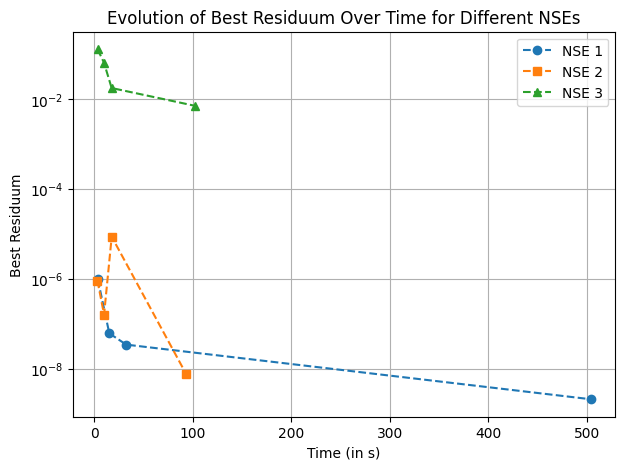
\includegraphics[width=0.45\textwidth]{Bilder/BestResiduum_Time_nse1-3.png}
		%\caption{Darstellung der besten\\ gefundenen Residuen über die Zeit}
		\label{fig:bestresiduum_time_allnse}
	\end{subfigure}
	\hfill
	\begin{subfigure}
		\centering
		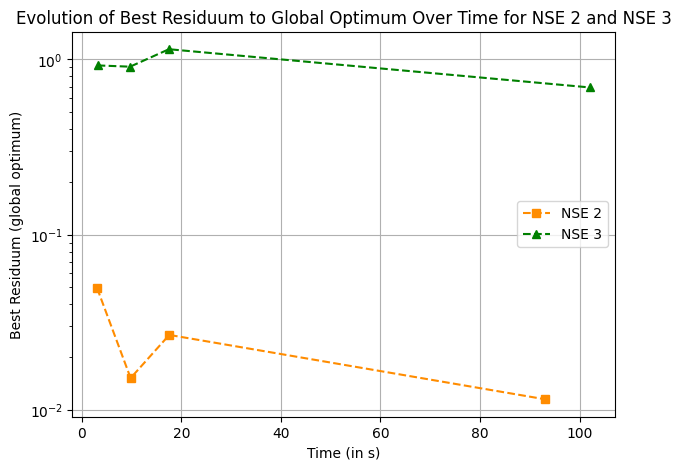
\includegraphics[width=0.45\textwidth]{Bilder/Residuum_globaloptimum_time_nse2-3.png}
		%\caption{Darstellung der besten\\ gefundenen Residuen zum globalen\\ Optimum über die Zeit}
		\label{fig:bestresiduum_globaloptimum_time_nse1-2}
	\end{subfigure}
	\caption{Darstellung der besten gefundenen Residuuen über die Zeit für alle Probleme und der besten Residuen zum globalen Optimum für NSE 1 \& NSE 2}
	\label{fig:zusammenstellung}
\end{figure}

\begin{figure}[h]
	\centering
	\begin{subfigure}
		\centering
		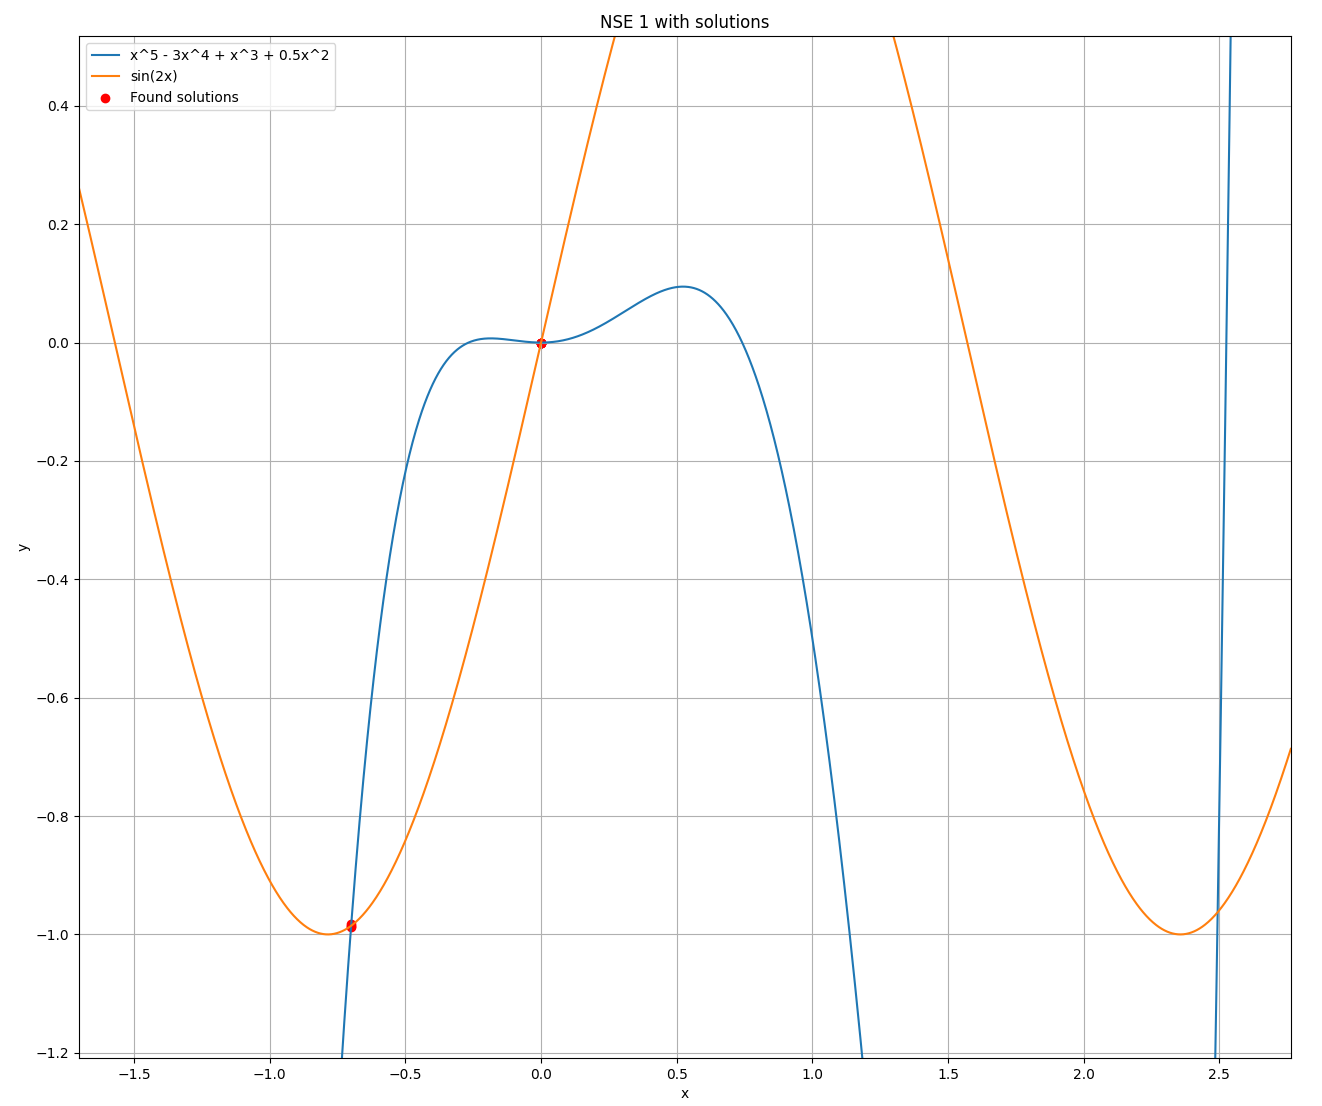
\includegraphics[width=0.45\textwidth]{Bilder/solutions_nse1.png}
		%\caption{Gefundene Lösung für NSE 1 (\ref{nse:1}) mit einem Schwellenwert $\leq 1e-5$}
		\label{fig:solutions_nse1}
	\end{subfigure}
	\hfill
	\begin{subfigure}
		\centering
		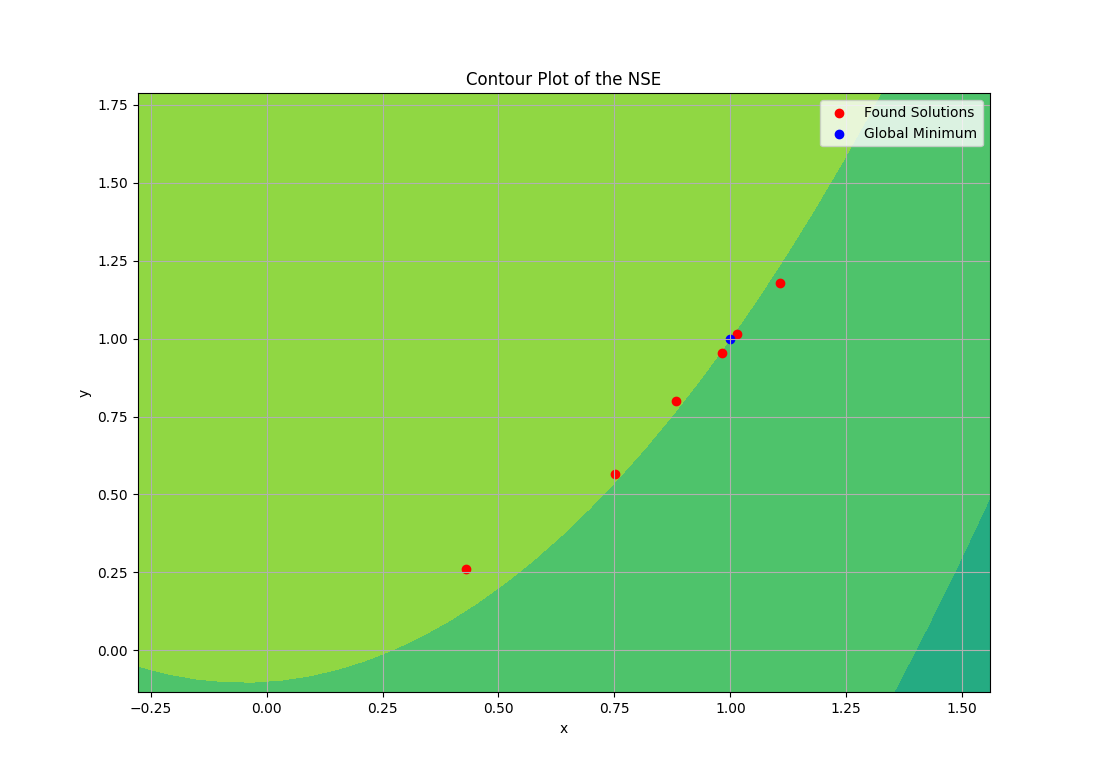
\includegraphics[width=0.45\textwidth]{Bilder/solutions_nse2.png}
		%\caption{Gefundene Lösung für NSE 2 (\ref{nse:2}) mit einem Schwellenwert $\leq 1e-3$}
		\label{fig:solutions_nse2}
	\end{subfigure}
	\caption{Gefundene Lösungen für NSE 1 (mit Schwellenwert $\leq 1e-5$) und NSE 2 (mit Schwellenwert $\leq 1e-3$)}
	\label{fig:solutions_nse1_nse2}
\end{figure}


In den vorliegenden Ergebnissen fällt besonders auf, dass das vermeintlich einfachste Problem (NSE 1, \ref{nse:1}) die längste Zeit benötigt, um alle 50.000 Epochen abzuschließen - etwa 500 Sekunden. Im Gegensatz dazu liegt die Dauer für die Absolvierung der gleichen Anzahl von Epochen für die Probleme \ref{nse:rosenbrock} und \ref{nse:highdimension} in einer Größenordnung von nur knapp 100 Sekunden. Eine mögliche Erklärung dafür liegt darin, dass das Residuum für das erste Problem (NSE 1, \ref{nse:1}) sehr schnell in einen extrem kleinen Bereich fällt. Dadurch erfordert selbst eine geringfügige Verbesserung des Ergebnisses bereits sehr kleine Anpassungen in den Aktionen des Agenten. Allerdings könnte der Agent aufgrund von Beschränkungen in seiner Aktionsraumgröße Schwierigkeiten haben, Änderungen im Bereich von $1e-9$ zu erreichen. Dadurch wird möglicherweise keine signifikante Verbesserung erzielt, sodass die Optimierung stagniert und die Zeit zur Absolvierung der 50000 Epochen zunimmt. 

Jedoch wäre dies nur eine anfängliche Idee, die tiefer untersucht werden müsste, da für die Konvergenz des Verfahrens viele weitere Parameter einen Einfluss ausüben.
\medskip

Bei Problem 1 (NSE 1 \ref{nse:1}) ist zudem die Besonderheit, dass das nichtlineare Gleichungssystem mehrere globale Optima besitzt (in diesem Fall genau drei). Die meisten Verfahren, wie zum Beispiel das Newton-Raphson-Verfahren benötigen einen anfänglichen Startpunkt, und nähern sich dann iterativ genau \textbf{einer} Lösung an, sofern sie denn existiert. Beim vorliegenden Verfahren ist die Besonderheit, dass zum Teil mehrere Lösungen gefunden werden können, da der Agent allein lernt, das negative Residuum (Belohnung) zu maximieren. Da für alle Lösungen gilt, dass das Residuum $= 0$ ist, können entsprechend auch mehrere Lösungen gleichzeitig mit einer hinreichenden Genauigkeit gefunden werden. In mehreren Testläufen wurde auch die Lösung $x^{\ast} \approx -0.6998$ mit einer Genauigkeit, die sich in einer Größenordnung von $1e-7$ befindet, gefunden. In den seltensten Fällen jedoch wurde die Lösung bei $x^{\ast} \approx 2.4936$ mit einer Genauigkeit von $\leq 1e-5$ gefunden. Grund dafür ist die große Sensibilität beim Residuum, denn in diesem Bereich weist die Funktion $f(x) = x^5 - 3x^4+x^3+0.5x^2$ eine große Steigung auf, sodass kleine Änderungen im Wert von $x$ hier zu erheblichen Änderungen im Funktionswert $y$ führen. Dies hat zur Folge, dass die Belohnung für kleinere Änderungen in der Aktion stärker schwankt, sodass diese Aktionen im Mittel nicht vielversprechend genug sind. Der Agent konzentriert sich dann eher auf die Aktionen, die im Mittel eine höhere Belohnung liefern, sodass der Agent diese auch weiter verfolgt und in der näheren Umgebung dieser Aktionen mehr erkundet.

In der Abbildung \ref{fig:reward-action-nse1-logscale} wird deutlich, wie sich die Belohnung in Abhängigkeit von der gewählten Aktion verhält.

Dort ist deutlich zu sehen, dass die Belohnung spärlich um das eigentliche globale Optimum bei $x^{\ast} \approx 2.4936$ verteilt ist, sodass der Agent diese Aktion nicht genug bevorzugt und die Lösung nicht mit erhöhter Genauigkeit gefunden werden kann.

\begin{figure}[h]
	\centering
	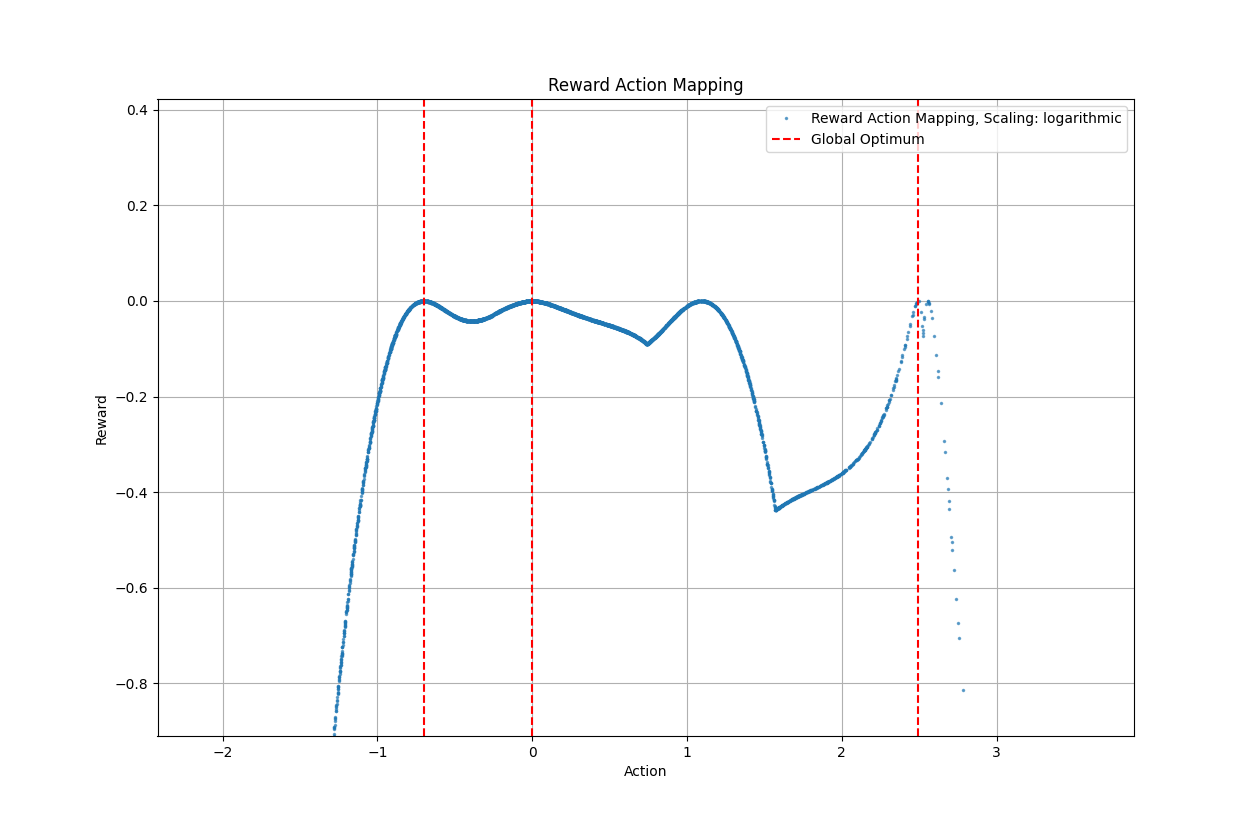
\includegraphics[width=0.5\textwidth]{Bilder/reward_action_nse1_logscale.png}
	\caption{Belohnung in Abhängigkeit von der Aktion für NSE 1 (\ref{nse:1}). Logarithmische Skalierung des Residuums}
	\label{fig:reward-action-nse1-logscale}
\end{figure}
\medskip

Des Weiteren ist bei NSE 2 (\ref{nse:rosenbrock}) zu erkennen, dass bei einer Epochen-Anzahl von $10000$ die beste gefundene Aktion schlechter ist als im Vergleich dazu die beste gefundene Aktion bei einer geringeren Epochen-Anzahl wie $1000$. 

Die könnte mit der Zufälligkeit des Agenten zusammenhängen, da der Agent zu Beginn zufällig im gegebenen Raum initialisiert wird und auch mit jedem Aufruf der \code{reset} Methode zufällig zurückgesetzt wird.

Zudem wird auch hier die Problematik des nichtlinearen Gleichungssystems deutlich. Die Rosenbrock-Funktion besteht aus einem \glqq Banana\grqq{}-förmigen Tal mit mehreren lokalen Optima, sodass viele Optimierungsverfahren Schwierigkeiten haben das globale Optimum zu finden. Von dieser Problematik ist auch dieses Verfahren nicht ausgeschlossen. Der Agent findet zwar Lösungen mit einer Genauigkeit, die sich in einer Größenordnung von $1e-8$ befinden, jedoch sind diese zumeist lokale Optima, die beliebig weit vom globalen Optima entfernt sein können. Aus diesem Grund wurde auch die Spalte \textit{Best Action (Global Optimum)} (mit dem zugehörigen Residuum in der Spalte \textit{Best Residuum (Global Optimum)}) der Tabelle \ref{tab:Ergebnisse} hinzugefügt, um die Aktion zu betrachten, die sich am nächsten zum tatsächlichen globalen Optimum befindet. Werden diese zwei Spalten für die beiden Probleme (\ref{nse:rosenbrock} \& \ref{nse:highdimension}) betrachtet, lässt sich erkennen, dass das Residuum für diese Aktionen deutlich höher ist als das Residuum für die beste gefundenen Aktion.
\medskip

Es ist nicht überraschend, dass die Genauigkeit der Lösung für NSE 3 (\ref{nse:highdimension}) bei gleicher Anzahl an Epochen geringer ist. Dies liegt daran, dass der Aktionsraum in diesem Fall 10-dimensional ist. Der Agent hat daher Schwierigkeiten, die Richtung zu bestimmen, in der sich das Residuum verbessern könnte. Mit steigender Dimension könnte sich diese Problematik weiter verschärfen, sodass der Agent bzw. der grundlegende Algorithmus für diese Problemstellung optimiert werden muss.
\medskip

Grundlegend bei RL ist vor allen Dingen die \glqq teure\grqq{} Berechnung. Da der PPO-Algorithmus verwendet wurde, müssen dabei in jedem Schritt zwei neuronale Netze aktualisiert werden (Actor- und Critic-Netzwerk). Dies ist insbesondere im Vergleich zum relativ simplen Newton-Raphson-Verfahren sehr teuer und ein nicht zu vernachlässigender Faktor, der sich auf die Zeit auswirkt, bis zu dem eine Lösung mit einer bestimmten Genauigkeit gefunden wird.
\\

In diesem Kapitel wurden die wichtigsten Ergebnisse vorgestellt, die mit dem Ansatz erzielt wurden und untereinander verglichen. Es wurde auf Besonderheiten eingegangen und versucht mögliche Erklärungen zu finden. Abschließend dazu folgt nun das Fazit.


\section{Fazit}

Als Fazit kann formuliert werden, dass das präsentierte Verfahren grundsätzlich in der Lage ist Lösungen von nichtlinearen Gleichungssystemen zu finden. Besonders gut funktioniert das Verfahren für eindimensionale Probleme, bei denen die Lösungen robust sind, als nicht sensibel auf kleine Änderungen der Aktion reagieren. Anders formuliert funktioniert das Verfahren eben für solche eindimensionale nichtlineare Gleichungssysteme gut, bei denen die Summe der Beträge der Steigungen aller Gleichungen klein ist. Für solche Probleme ist das Verfahren mit dargestellter Umsetzung in der Lage Lösungen mit einer Genauigkeit von $1e-8$ bis zu $1e-9$ zu finden. Vor dem Hintergrund der Zeit und der Berechnungskomplexität allerdings, schließt dieses Verfahren insbesondere im Vergleich zu dem etablierten Newton-Raphson-Verfahren schlecht ab. Dieses Verfahren findet mit weniger Berechnungen und in kürzerer Dauer die Lösung mit einer höheren Genauigkeit. Jedoch sollte dabei auch erwähnt sein, dass dieses Verfahren einen initialen Startpunkt benötigt, von dem das Verfahren sich iterativ der nächsten Lösung annähert. Demzufolge auch nur eine Lösung findet. 

Es hängt vom spezifischen Anwendungsfall ab, ob es genügt eine Lösung zu finden, oder mehr. Sollte der Fall vorliegen, dass mehrere Lösungen gefunden werden sollen, so könnte das hier präsentierte Verfahren geeigneter sein als das Newton-Raphson-Verfahren, sofern auch die zeitliche Komponente keine große Rolle spielt. Zusätzlich dazu kann das hier vorgestellte Verfahren möglicherweise eher dazu verwendet werden, eine oder mehrere mögliche Startpunkte für andere iterative Verfahren zu generieren, wenn keinerlei Informationen über die grobe Lage von Lösungen vorliegt. Die iterativen Verfahren könnten im Anschluss daran die bisherigen gefundenen Lösungen nutzen, um diese weiter zu verbessern und schnell eine Lösung größerer Genauigkeit zu finden.
\medskip

Bei der Anwendung dieses Verfahrens auf die Rosenbrock-Funktion (NSE 2, \ref{nse:rosenbrock}), wurde deutlich, dass auch dieses Verfahren Schwierigkeiten hat, das globale Optimum zuverlässig zu finden. Wie viele andere Optimierungsalgorithmen ist es anfällig für das Feststecken in lokalen Optima, was seine Fähigkeit zur zielgerichteten Suche nach dem globalen Optimum einschränkt. Diese Herausforderung betrifft eine Vielzahl von Optimierungsmethoden und erfordert eine kontinuierliche Verbesserung, um damit umzugehen. Zusätzliche Informationen, die spezifisch für das Problem sind, können helfen, das globale Optimum besser und effizienter zu finden. Allerdings könnten solche Informationen für andere Problemstellungen weniger relevant sein, was ihre breite Anwendbarkeit einschränken könnte.
\medskip

Insbesondere bei nichtlinearen Gleichungen höherer Dimension deutet sich an, dass die Genauigkeit der gefundenen Lösungen stark abnimmt. Während für NSE 1 und NSE 2 Lösungen mit einer Genauigkeit von $1e-7$ bis $1e-9$ gefunden werden konnten, befand sich die beste gefundene Lösung für NSE 3 (mit einer Dimension von  $10$) in einer Größenordnung von $1e-3$ bei gleichbleibender Epochen-Anzahl.

Es bleibt zu untersuchen, ob eine generelle Tendenz besteht, dass die Genauigkeit der Lösung mit zunehmender Dimension des Problems abnimmt. Um diese Frage zu beantworten, sind ausführliche Tests und Untersuchungen erforderlich, die eine umfassende Analyse der Leistung des Reinforcement-Learning-Agenten in Bezug auf verschiedene Problemgrößen ermöglichen. Erst nach gründlicher Analyse und Evaluation können valide Schlussfolgerungen gezogen werden.
\\

Abschließend ist anzumerken, dass neben den bereits diskutierten Parametern eine Vielzahl weiterer Faktoren die Lösungsfindung und die Qualität der Lösung beeinflussen können. Diese zusätzlichen Faktoren können die Effektivität des Verfahrens beeinträchtigen und sollten daher ebenfalls berücksichtigt werden. Dazu gehören:

\begin{itemize}
	\item Die Größe des Aktionsraumes
	\item Die Definition des Zustandes
	\item Die Berechnung und Skalierung des Residuums
	\item Die Gestaltung der Belohnungsfunktion
	\item Der zugrunde liegende RL-Algorithmus mit allen zugehörigen beeinflussbaren Hyperparametern, wie Lernrate, Batch-Size usw.
\end{itemize}

Zusätzlich zu den diskutierten Parametern beeinflussen eine Vielzahl weiterer Faktoren die Lösungsfindung und -qualität. Eine tiefere Analyse des Einflusses dieser Parameter in Bezug auf die spezifische Problemstellung ist daher von entscheidender Bedeutung.

Diese Arbeit bietet somit Einblicke in die Möglichkeiten und Herausforderungen bei der Anwendung von Reinforcement Learning zur Lösung nichtlinearer Gleichungssysteme und legt den Grundstein für weitere Untersuchungen auf diesem Gebiet. 


\newpage

\clearpage % or \cleardoublepage

\addcontentsline{toc}{section}{Literaturverzeichnis}

\printbibliography

\newpage

\section{Eigenständigkeitserklärung}

Ich habe diese Arbeit selbstständig und ohne fremde Hilfe Dritter angefertigt. Bei der Übernahme fremder Gedanken habe ich dies als Zitat kenntlich gemacht. 

Bielefeld, 06.04.2024

Nicolas Schneider

\end{onehalfspace}

\end{document}








